\begin{figure}
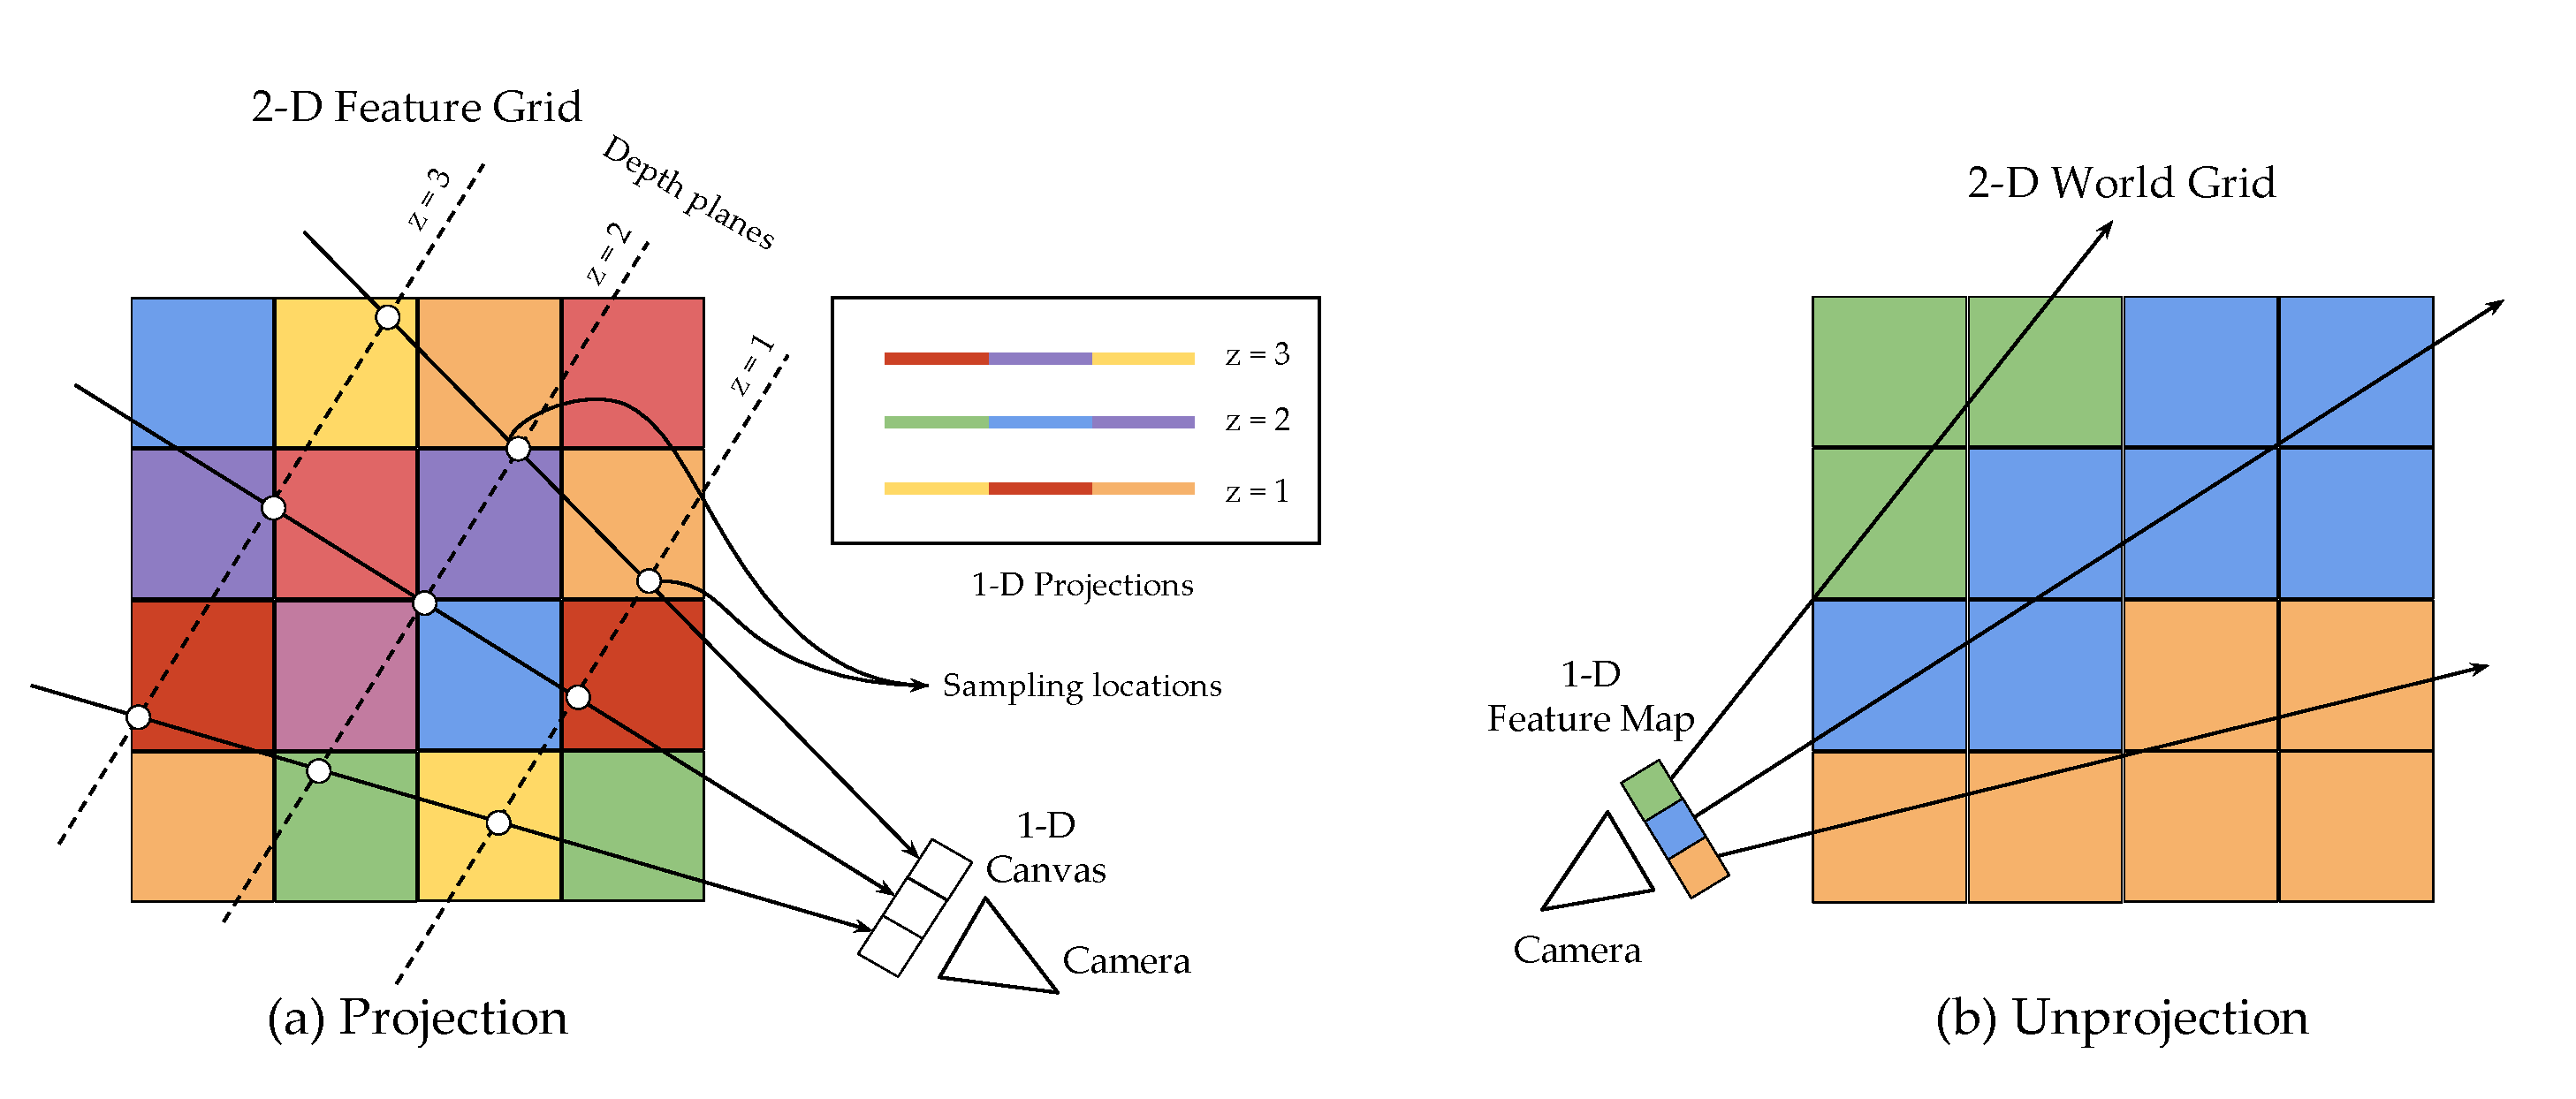
\includegraphics[width=0.95\linewidth]{figures/lsm/proj_unproj.pdf}
\caption{Illustrations of projection and unprojection operations between 1D maps and 2D grids. (a) The projection operation samples values along the ray at equally spaced z-values into a 1D canvas/image. The sampled features (shown by colors here) at the z planes are stacked into channels to form the projected feature map. (b) The unprojection operation takes features from a feature map (here in 1-D) and places them along rays at grid blocks where the respective rays intersect. Best viewed in color.}
\figlabel{proj_unproj}
\end{figure}